% Slides de la présentation préliminaire A1 (5 minutes), groupe 40 « La piscine ».
% Compilation (depuis slides/) : pdflatex slides.tex, puis copier slides.pdf à la racine du dépôt.
% Les figures sont lues dans ../figures/ (produites par experiments/*.py).
\documentclass[aspectratio=169,10pt]{beamer}

\usepackage[T1]{fontenc}
\usepackage[utf8]{inputenc}
\usepackage[french]{babel}
\usepackage{lmodern}
\usepackage{amsmath,amssymb}
\usepackage{booktabs}
\usepackage{tikz}

\graphicspath{{../figures/}}

\definecolor{accent}{HTML}{2A6FDB}
\definecolor{warm}{HTML}{E8833A}
\definecolor{ok}{HTML}{1A9E5C}
\definecolor{ink}{HTML}{222222}

\usetheme{default}
\setbeamertemplate{navigation symbols}{}
\setbeamercolor{frametitle}{fg=accent}
\setbeamercolor{title}{fg=accent}
\setbeamercolor{normal text}{fg=ink}
\setbeamercolor{structure}{fg=accent}
\setbeamerfont{frametitle}{series=\bfseries, size=\Large}
\setbeamertemplate{itemize item}{\color{accent}$\blacktriangleright$}
\setbeamertemplate{footline}{\hfill\textcolor{gray}{\scriptsize\insertframenumber/\inserttotalframenumber}\hspace{1em}\vspace{0.6em}}

\newcommand{\R}{\mathbb{R}}
\newcommand{\rhat}{\hat r}
\newcommand{\key}[1]{\textcolor{accent}{\textbf{#1}}}

\title{Que peut-on apprendre au-delà des biais ?}
\subtitle{Complétion d'une matrice de notes MovieLens très creuse}
\author{Groupe 40 --- La piscine}
\institute{DataLab A1 --- Master IASD}
\date{15 octobre 2026}

\begin{document}

%-----------------------------------------------------------------------------
\begin{frame}
\titlepage
\end{frame}

%-----------------------------------------------------------------------------
\begin{frame}{Le problème}
\begin{columns}[T]
\column{0.52\textwidth}
\begin{itemize}
  \item Matrice $R$ : \key{610 utilisateurs $\times$ 4\,980 films}, notes de 0,5 à 5
  \item Seules \key{1\,\%} des cases sont connues
  \item Objectif : prédire toutes les autres, évaluées en
\end{itemize}
\[
  \mathrm{RMSE} = \sqrt{\tfrac{1}{|T|} \textstyle\sum_{(u,i)\in T} (r_{ui} - \rhat_{ui})^2}
\]
\column{0.45\textwidth}
\small
\begin{tabular}{@{}lll@{}}
\toprule
 & \textbf{Entrée} & \textbf{Score} \\
\midrule
Local      & train         & test \\
Plateforme & train + test  & eval (caché) \\
\bottomrule
\end{tabular}

\vspace{1em}
Contraintes : CPU, 4 threads, 1\,200\,s.
\end{columns}

\vspace{1.2em}
\begin{center}
\colorbox{accent!8}{\parbox{0.85\textwidth}{\centering
\textbf{Question :} une fois les biais utilisateur et film retirés,\\
reste-t-il un signal exploitable ?}}
\end{center}
\end{frame}

%-----------------------------------------------------------------------------
\begin{frame}{Les données : très creuses, peu de structure au-delà des biais}
\begin{columns}[T]
\column{0.40\textwidth}
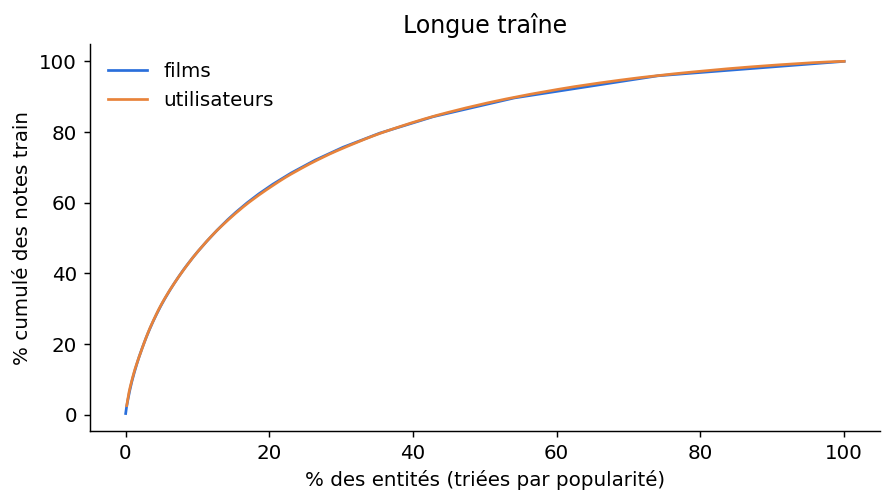
\includegraphics[width=\linewidth]{eda/03_long_tail.png}
\column{0.58\textwidth}
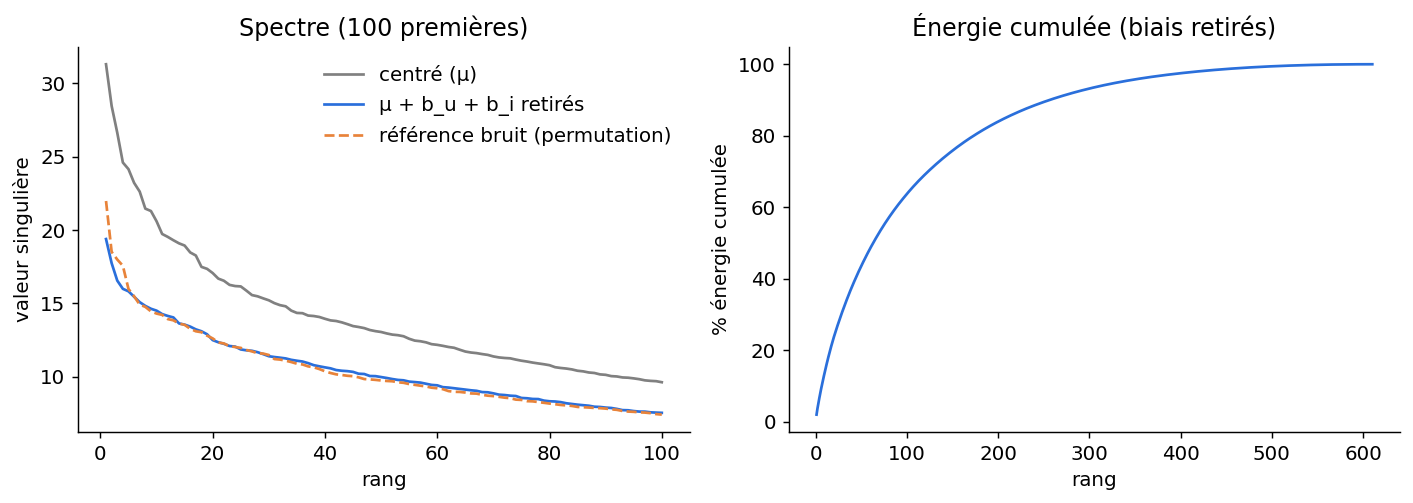
\includegraphics[width=\linewidth]{eda/10_svd_spectrum.png}
\end{columns}
\vspace{0.4em}
\begin{itemize}
  \item Un film a \key{3 notes} en médiane ; 21\,\% des notes de test portent sur un film à moins de 5 notes
  \item Biais seuls : RMSE $1{,}037 \to \key{0{,}875}$
  \item Résidus : spectre indiscernable d'un bruit permuté au-delà du rang $\approx 5$
\end{itemize}
\end{frame}

%-----------------------------------------------------------------------------
\begin{frame}{Protocole expérimental}
\begin{center}
\begin{tikzpicture}[x=1cm,y=1cm]
  \fill[accent!70] (0,0) rectangle (8.1,0.7);
  \fill[warm!80] (8.1,0) rectangle (9.3,0.7);
  \fill[gray!45] (9.8,0) rectangle (13.8,0.7);
  \node[white] at (4.05,0.35) {\small\textbf{train 90\,\%} : apprentissage};
  \node[white] at (8.7,0.35) {\small\textbf{valid.}};
  \node at (11.8,0.35) {\small\textbf{test}};
  \node[above] at (4.05,0.75) {\small\textcolor{gray}{train (31\,598 notes)}};
  \draw[->,thick,warm] (8.7,-0.1) to[bend left=12] node[below,text=ink]{\small choix des hyperparamètres} (4.05,-0.1);
  \node[below] at (11.8,-0.1) {\small \textbf{une seule} évaluation finale};
\end{tikzpicture}
\end{center}
\vspace{0.6em}
\begin{itemize}
  \item Meilleure configuration réentraînée sur tout le train, \key{test jamais utilisé pour régler}
  \item Mesures : RMSE, accuracy (note exacte après arrondi), temps d'entraînement
  \item Analyse par popularité du film : \emph{où} chaque méthode aide-t-elle ?
  \item Même interface pour tous les modèles : \texttt{fit(train) $\to$ predict(u, i)}
\end{itemize}
\end{frame}

%-----------------------------------------------------------------------------
\begin{frame}{Méthodes comparées}
\footnotesize
\begin{tabular}{@{}p{3.1cm}p{9.9cm}@{}}
\key{Biais} (baseline) &
  $\rhat_{ui} = \mu + b_u + b_i$, \; pénalité $\lambda \bigl(\|b_u\|^2 + \|b_i\|^2\bigr)$ \\[6pt]
\key{Factorisation} &
  $\rhat_{ui} = \mu + b_u + b_i + p_u^\top q_i$, \; pénalités séparées $\lambda_b$, $\lambda_f$ \\
  & ALS : $p_u = (Q_u^\top Q_u + \lambda_f I)^{-1} Q_u^\top \tilde r_u$ \quad / \quad SGD \\[6pt]
\key{Soft-Impute} &
  $\min_Z \tfrac12 \sum_{\text{obs.}} (r_{ui} - z_{ui})^2 + \tau \|Z\|_*$ : seuillage des valeurs singulières \\[6pt]
\key{$k$NN films} &
  $\rhat_{ui} = \text{biais} + \dfrac{\sum_{j \in N_k(i;u)} s_{ij}\, e_{uj}}{\beta + \sum_j |s_{ij}|}$, \;
  Pearson rétréci $s_{ij}\tfrac{n_{ij}}{n_{ij}+100}$ \\[10pt]
\key{Biais + genres} &
  $b_i$ tiré vers $f_i^\top w$ (genres, décennie, popularité) au lieu de 0 \\[6pt]
\key{Mélange} &
  régression ridge sur la validation : $\rhat_{ui} = w_0 + \sum_m w_m \rhat^{(m)}_{ui}$ \\[6pt]
\key{AutoRec} (deep) &
  $\hat{\boldsymbol e}_{\cdot i} = V\,\sigma(W \boldsymbol e_{\cdot i} + b) + c$ sur les résidus des biais, perte sur les notes observées \\[6pt]
\key{MF bayésienne} &
  a priori sur facteurs et régularisation, échantillonnage de Gibbs, $\rhat_{ui} = \tfrac1S \sum_s \rhat^{(s)}_{ui}$ \\
  & \textbf{FM} : + films notés par $u$ (SVD++), + utilisateurs ayant noté $i$, + genres \\
\end{tabular}
\end{frame}

%-----------------------------------------------------------------------------
\begin{frame}{Factorisation : tout se joue dans la régularisation}
\begin{center}
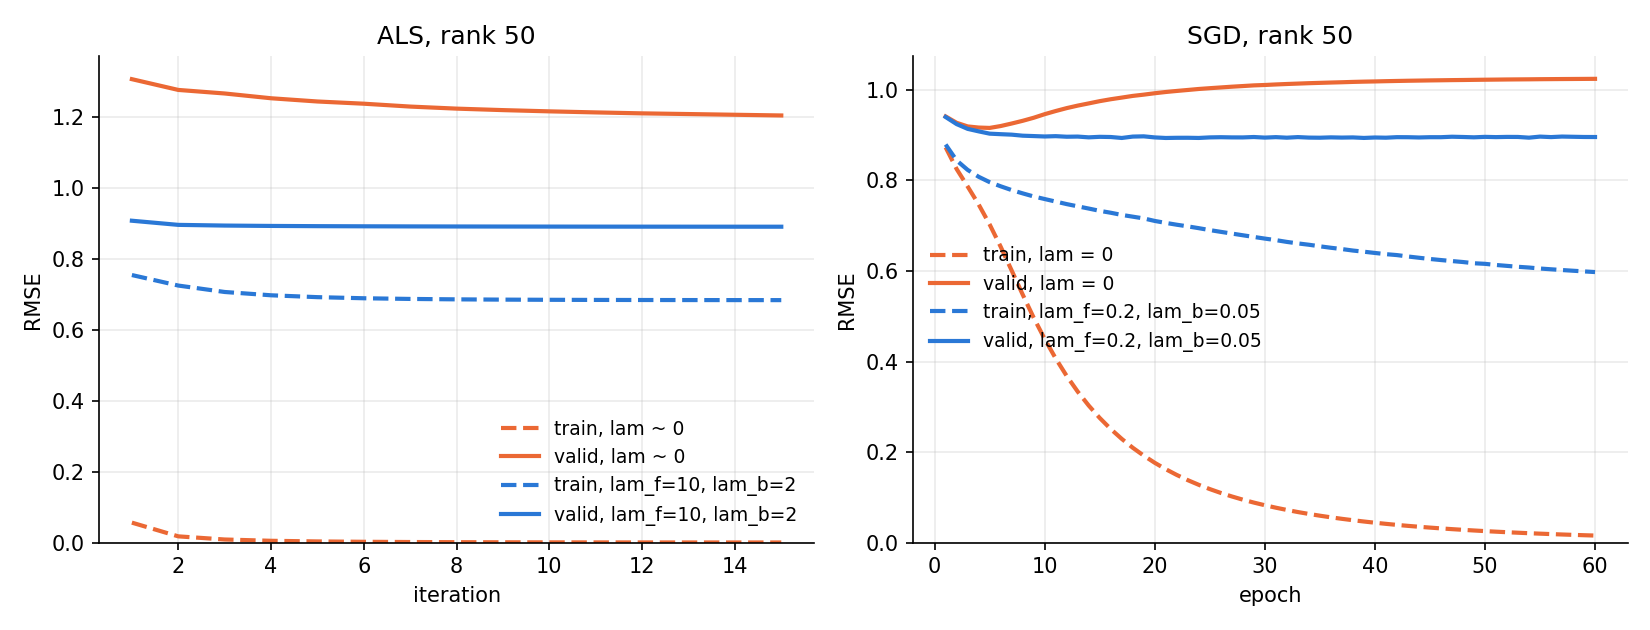
\includegraphics[width=0.78\linewidth]{mf_learning_curves.png}
\end{center}
\begin{itemize}
  \item Sans régularisation : RMSE train $\to 0$, validation $> 1{,}0$ (surapprentissage)
  \item $\lambda_f \geq 15$ : facteurs écrasés, on retombe exactement sur les biais
  \item Fenêtre utile étroite ($\lambda_f \approx 10$) ; ensuite le rang compte peu
\end{itemize}
\end{frame}

%-----------------------------------------------------------------------------
\begin{frame}{MF bayésienne : moyenner plutôt qu'optimiser}
\begin{columns}[T]
\column{0.55\textwidth}
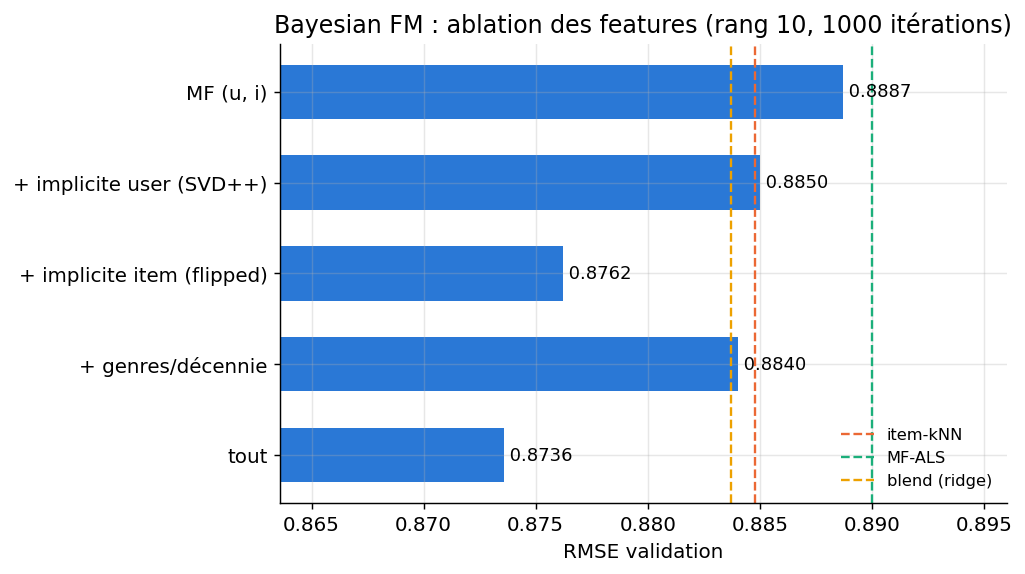
\includegraphics[width=\linewidth]{bayes/ablation.png}
\column{0.43\textwidth}
\vspace{0.6em}
\begin{itemize}
  \item Un échantillon seul : RMSE $\approx 1{,}03$ ; la \key{moyenne} de 2\,000 : $0{,}873$
  \item La régularisation est \key{apprise} : plus de $\lambda$ à régler
  \item Le plus utile : savoir \key{qui a noté le film}, pas la note elle-même
  \item Genres : petit gain, cumulable
\end{itemize}
\end{columns}
\end{frame}

%-----------------------------------------------------------------------------
\begin{frame}{Résultats}
\begin{columns}[T]
\column{0.42\textwidth}
\small
\begin{tabular}{@{}lcr@{}}
\toprule
\textbf{Méthode} & \textbf{RMSE test} & \textbf{s} \\
\midrule
Moyenne globale     & 1,037 & 0 \\
Biais               & 0,875 & 0,01 \\
MF -- SGD           & 0,878 & 0,5 \\
MF -- ALS           & 0,873 & 1,5 \\
Soft-Impute         & 0,872 & 4,7 \\
AutoRec             & 0,872 & 17 \\
$k$NN films         & 0,871 & 1,1 \\
Mélange             & 0,868 & 7,7 \\
BPMF                & 0,865 & 44 \\
\midrule
\textbf{FM bayésienne} & \textbf{0,855} & 60 \\
\bottomrule
\end{tabular}

\column{0.54\textwidth}
\vspace{1em}
\begin{itemize}
  \item Méthodes \og ponctuelles \fg{} : moins de \key{0,01} de gain sur les biais
  \item AutoRec (deep) : aucun gain, surapprend fortement
  \item MF bayésienne : \key{$-0{,}019$}, le seul saut net
  \item FM bayésienne : \key{93\,s} sur train + test, loin des 1\,200\,s
\end{itemize}
\end{columns}
\end{frame}

%-----------------------------------------------------------------------------
\begin{frame}{Où chaque méthode aide-t-elle ?}
\begin{center}
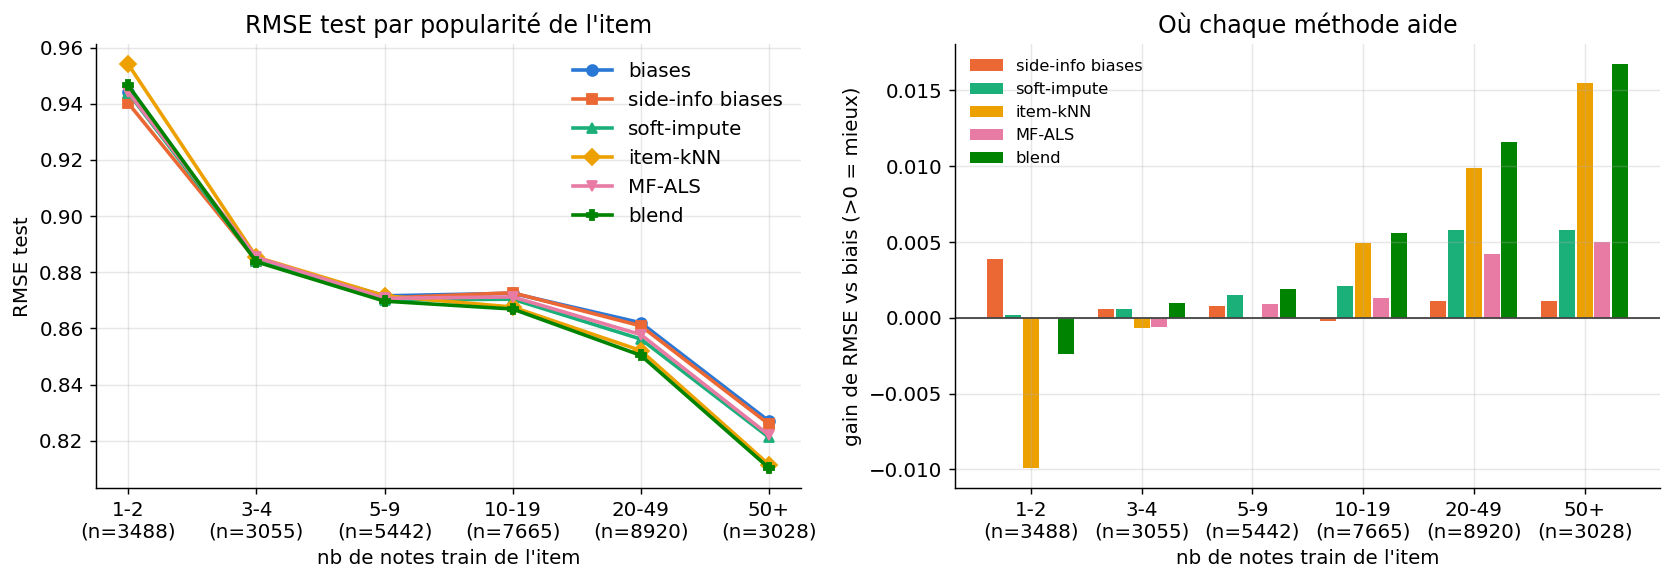
\includegraphics[width=0.95\linewidth]{alt/rmse_by_popularity.png}
\end{center}
\begin{itemize}
  \item $k$NN et Soft-Impute gagnent sur les films \key{populaires} (jusqu'à $-0{,}016$)
  \item Sur les films à \key{1--2 notes}, seuls les biais guidés par les genres aident
\end{itemize}
\end{frame}

%-----------------------------------------------------------------------------
\begin{frame}{Leçons et suite}
\begin{columns}[T]
\column{0.5\textwidth}
\textbf{Ce que nous avons appris}
\begin{itemize}
  \item À 1\,\% de densité, \key{les biais font 90\,\%} du gain
  \item La formule $k$NN du cours surcorrige avec peu de voisins : $\beta = 0{,}2$ au dénominateur suffit
  \item Arrondir les prédictions : accuracy inchangée, RMSE $+0{,}012$
  \item Sur données creuses, \key{bayésien $>$ deep}
\end{itemize}
\column{0.5\textwidth}
\textbf{Prochaines étapes}
\begin{itemize}
  \item FM bayésienne dans \texttt{generate.py} (score plateforme)
  \item Mélange FM + $k$NN + BPMF
  \item Validation croisée sur train + test : les réglages tiennent-ils avec $2\times$ plus de notes ?
\end{itemize}
\end{columns}
\end{frame}

\end{document}
